%% RiSE Latex Template - version 0.5
%%
%% RiSE's latex template for thesis and dissertations
%% http://risetemplate.sourceforge.net
%%
%% (c) 2012 Yguaratã Cerqueira Cavalcanti (yguarata@gmail.com)
%%          Vinicius Cardoso Garcia (vinicius.garcia@gmail.com)
%%
%% This document was initially based on UFPEThesis template, from Paulo Gustavo
%% S. Fonseca.
%%
%% ACKNOWLEDGEMENTS
%%
%% We would like to thanks the RiSE's researchers community, the 
%% students from Federal University of Pernambuco, and other users that have
%% been contributing to this projects with comments and patches.
%%
%% GENERAL INSTRUCTIONS
%%
%% We strongly recommend you to compile your documents using pdflatex command.
%% It is also recommend use the texlipse plugin for Eclipse to edit your documents.
%%
%% Options for \documentclass command:
%%         * Idiom
%%           pt   - Portguese (default)
%%           en   - English
%%
%%         * Text type
%%           bsc  - B.Sc. Thesis
%%           msc  - M.Sc. Thesis (default)
%%           qual - PHD qualification (not tested yet)
%%           prop - PHD proposal (not tested yet)
%%           phd  - PHD thesis
%%
%%         * Media
%%           scr  - to eletronic version (PDF) / see the users guide
%%
%%         * Pagination
%%           oneside - unique face press
%%           twoside - two faces press
%%
%%		   * Line spacing
%%           singlespacing  - the same as using \linespread{1}
%%           onehalfspacing - the same as using \linespread{1.3}
%%           doublespacing  - the same as using \linespread{1.6}
%%
%% Reference commands. Use the following commands to make references in your
%% text:
%%          \figref  -- for Figure reference
%%          \tabref  -- for Table reference
%%          \eqnref  -- for equation reference
%%          \chapref -- for chapter reference
%%          \secref  -- for section reference
%%          \appref  -- for appendix reference
%%          \axiref  -- for axiom reference
%%          \conjref -- for conjecture reference
%%          \defref  -- for definition reference
%%          \lemref  -- for lemma reference
%%          \theoref -- for theorem reference
%%          \corref  -- for corollary reference
%%          \propref -- for proprosition reference
%%          \pgref   -- for page reference
%%
%%          Example: See \chapref{chap:introduction}. It will produce 
%%                   'See Chapter 1', in case of English language.

\documentclass[en,twoside,onehalfspacing,bsc]{risethesis}

\usepackage{natbib}
\usepackage{babel}
\usepackage{supertabular}
\usepackage{microtype}
\usepackage{lscape}

%% Change the following pdf author attribute name to your name.
\usepackage[linkcolor=blue,citecolor=blue,urlcolor=blue,colorlinks,pdfpagelabels,pdftitle={Bruno Cabral's Bachelor Thesis},pdfauthor={Bruno Cabral}]{hyperref}

\address{SALVADOR}

\universitypt{Universidade Federal da Bahia}
\universityen{Federal University of Bahia}

\departmentpt{Depertamento de Ci\^{e}ncia da Computa\c{c}\~{a}o}
\departmenten{Computer Science Department}

\programpt{Programa Multiinstitucional de P\'{o}s-gradua\c{c}\~{a}o em Ci\^{e}ncia da Computa\c{c}\~{a}o}
\programen{Graduate in Computer Science}

\majorfieldpt{Ci\^{e}ncia da Computa\c{c}\~{a}o}
\majorfielden{Computer Science}

\title{SPLICE: A flexible SPL lifecycle management tool}
\date{February/2014}

\author{Bruno Souza Cabral}
\adviser{Eduardo Santana de Almeida}
\coadviser{Tassio Ferreira Vale}

\begin{document}

\frontmatter
\frontpage
\presentationpage

\begin{dedicatory}
I dedicate this dissertation to my family, girlfriend, friends and
professors who gave me all necessary support to get here.
\end{dedicatory}

\acknowledgements
I would like to thank my beautiful family and friends. Especially to my dad, Charles, who always advised me and took care of all boring stuff in my life, so I could have time to concentrate; My mom, Eneida, who is a super mother, always worked insanely long periods and still have time to take care, cook and groom us; My sister, Debóra,  who had to handle my hugs and rants every half hour during my academic life. I truly love them and appreciate all the support they have given me. I would also like to express l my gratitude for my girlfriend, Bruna, for having an endless patience, and offering me a warm shoulder during my entire journey.

I would like to thanks Dr. Eduardo Almeida. He was the first professor to believe in my capacity, never gave up on me and kept me on the academic track during my times of doubt. He is someone who I truly admire and always been an inspirational figure for me. I also want to show all my gratitude to Dr. Cássio Prazeres for being an amazing advisor and for always being there during my graduation.

Finally, I would like to express my appreciation to Tassio Vale, my co-advisor, who pushed me to work, patiently revised my thesis multiple times and pointed me the way during the thesis writing.




\begin{epigraph}[]{Edward V Berard}
Walking on water and developing software from a specification are easy if both are frozen
\end{epigraph}

\resumo
% Escreva seu resumo no arquivo resumo.tex
O crescente aumento das tecnologias embutidas em dispositivos móveis (e.g. smartphones, tablets) e, seu uso cada vez mais constante na realização de diversas atividades do cotidiano (e.g. pagamento de contas, acesso à internet, acesso a mapas, gravação/reprodução de áudio e vídeo) tem alavancado o crescimento de aplicações que utilizam os recursos disponíveis no dispositivo móvel (e.g. Bluetooth, Wi-fi, GPS) e no ambiente em que esse se encontra (e.g. sensores de presença e temperatura, localização, data e hora, etc.). O objetivo é oferecer aos usuários serviços que tragam comodidade e praticidade em suas atividades diárias com o mínimo de interação explicita. Soluções computacionais neste domínio recebem o nome de aplicações sensíveis ao contexto e podem agregar excelentes aplicabilidades no cotidiano dos usuários. Neste contexto, constatando-se, através de estudos realizados, a necessidade de manter os usuários de transporte públicos bem informados acerca dos principais serviços de transportes disponíveis e, sobretudo, do que está acontecendo nas principais vias de uma determinada cidade,  este trabalho propõe a criação de um sistema mobile sensível ao contexto que, através da colaboração do usuário, possa propagar informações relacionadas a atual situação do trânsito e aos principais serviços do transporte público disponíveis (e.g. localização dos ônibus e pontos, rotas, horários, linhas e etc.), fazendo, desta forma, com que seus usuários tomem conhecimento em, praticamente, tempo real dos eventos de trânsito (e.g. acidentes, engarrafamentos, obras e etc.) que estão dificultando a mobilidade das vias que, possivelmente, eles utilizam para realizar suas atividades, seja ir ao trabalho, estudar, fazer compras ou, simplesmente, para o lazer. O foco é melhorar a informação oferecida aos usuários do transporte público, com base em informações fornecidas por outros indivíduos. 


\begin{keywords}
Computação Ubíqua, Computação Sensível ao Contexto, Inteligência Coletiva, \textit{Crowdsourcing}, Sistemas de Transporte Inteligentes, FindBus. 

\end{keywords}

\abstract
% Write your abstract in a file called abstract.tex


Software engineering is a discipline that integrates process, methods, and tools for the development of computer software. To support it, Application lifecycle management systems are software tools that assist in the organization and moderation of a project throughout its life cycle. There is an infinite number of possibilities to define a project life cycle, and the needed tools to help it completion. Consequently, a huge variety of management systems are available on today's market, specifically designed to conform to a diverse number of management methodologies. Nevertheless, most are proprietary, very specialized, with little to no customization, making very hard to find one that perfectly fit one's needs.

A different type of software systems development is Software Product Line Engineering -- SPLE. SPL is a methodology for developing a diversity of related software products and software-intensive systems. During the development of a SPL, a wide range of artifacts needs to be created and maintained to preserve the consistency of the family model during development, and it is important to manage the SPL variability and the traceability among those artifacts. However, this is a hard task, due to the heterogeneity of assets developed during product line engineering. Maintaining the traceability and artifacts updated manually is error-prone, time consuming and complex. Utilizing a tool for supporting those activities is essential. 

In this work, we propose the Software Product Line Integrated Construction Environment (SPLICE). That is a web-based life cycle management tool for managing, in an automated way, the software product line activities. This initiative intends to support most of the SPL process activities such as scoping, requirements, architecture, testing, version control, evolution, management and agile practices. This was archived with the integration of a framework around an established tool, providing an easy way for handling the usage of different metamodels.

We present a lightweight metamodel which integrates the processes of the SPL lifecycle agile practices, the implementation of a tool that uses the proposed metamodel, and a case study that reflect the feasibility and flexibility of this solution especially for different scenarios and processes



\begin{keywords}
software product line, agile, SPL, Application lifecycle management , tool, metamodel
\end{keywords}

% Summary (tables of contents)
\tableofcontents

% List of figures
\listoffigures

% List of tables
\listoftables

% List of acronyms
% Acronyms manual: http://linorg.usp.br/CTAN/macros/latex/contrib/acronym/acronym.pdf
\listofacronyms
\begin{acronym}[ACRONYM] 
% Change the word ACRONYM above to change the acronym column width.
% The column width is equals to the width of the word that you put.
% Read the manual about acronym package for more examples:
%   http://linorg.usp.br/CTAN/macros/latex/contrib/acronym/acronym.pdf




  \acro{IPEA}{Instituto de Pesquisa Econômica Aplicada}
  \acro{Denatran}{Departamento Nacional de Trânsito}
  \acro{IBGE}{Instituto Brasileiro de Geografia e Estatística}
    \acro{IDC}{IInternational Data Corporation}
        \acro{PLANTER}{Observatório do Comportamento \& Tendências}
    
\end{acronym}

% List of listings
%\lstlistoflistings

\mainmatter

\chapter{Trabalhos Relacionados}
\label{ch:trabalhosRelacionados}

Existem diversas plataformas que utilizam a LMS e gamificação para ensinar algum conteúdo a um grupo. Muitas dessas páginas Webs contém algumas semelhanças com a GameInfor. Contudo, mesmo sabendo que todas essas plataformas  têm como objetivo explicar uma temática através de uma série de etapas, elas possuem algumas importantes diferenças na sua proposta, essas diferenças podem definir o público alvo, o interesse do aluno nos tópicos passados e o custo benefício do uso de uma página específica.

Neste capítulo serão mostraremos algumas dessas plataformas, para cada uma delas apresentaremos as suas funcionalidades, o seu público alvo, seus pontos positivos e negativos. As plataformas que vamos abordar são: Engage, Apta, Moodle, Kaptiva e Dokeos.

\section{Engage}

A engage é uma plataforma de ensino que pode ser acessada através do link https://www.engage.bz, ela fornece ao usuário a possibilidade de criar uma série de cursos sobre os mais diversos conteúdos. Esta plataforma tem como público alvo as empresas que desejam fornecer aos seus funcionários cursos diversos. A ideia da mesma é que a empresas façam uso de seus recursos para passar os conhecimentos aos empregados.

Está é uma plataforma gamificada, ou seja, ela utiliza conceitos de jogos para tornar o conteúdo mais atraente aos funcionários que participarão do curso. Alguns dos conceitos utilizados são:

\begin{itemize}
\item Jogo de perguntas: nesses jogos são utilizadas animações para atrair visualmente o usuário, um relógio de pontos, nessa funcionalidade o usuário terá uma pontuação máxima para responder a pergunta, a medida que o tempo passar os pontos que serão recebidos caso a pergunta seja respondida de forma correta vai diminuindo.
\item Ranking: com essa funcionalidade o usuário pode competir amigavelmente com seus colegas de trabalho, verificando quem está obtendo a melhor pontuação no curso.
\item Conquistas pessoais: além de acompanhar o ranking geral de todos que estão fazendo o curso, a pessoa também pode acompanhar seu próprio andamento.
\item Avatar: o indivíduo pode também criar avatar escolhendo características como sexo, cor da pele, cabelo, olho, boca e nariz.
\end{itemize}

Resumindo, essa é uma boa plataforma, porém ela tem como desvantagem o fato de ser paga e ter um escopo de usuários limitada.

\begin{figure}[htp]
\begin{center}
  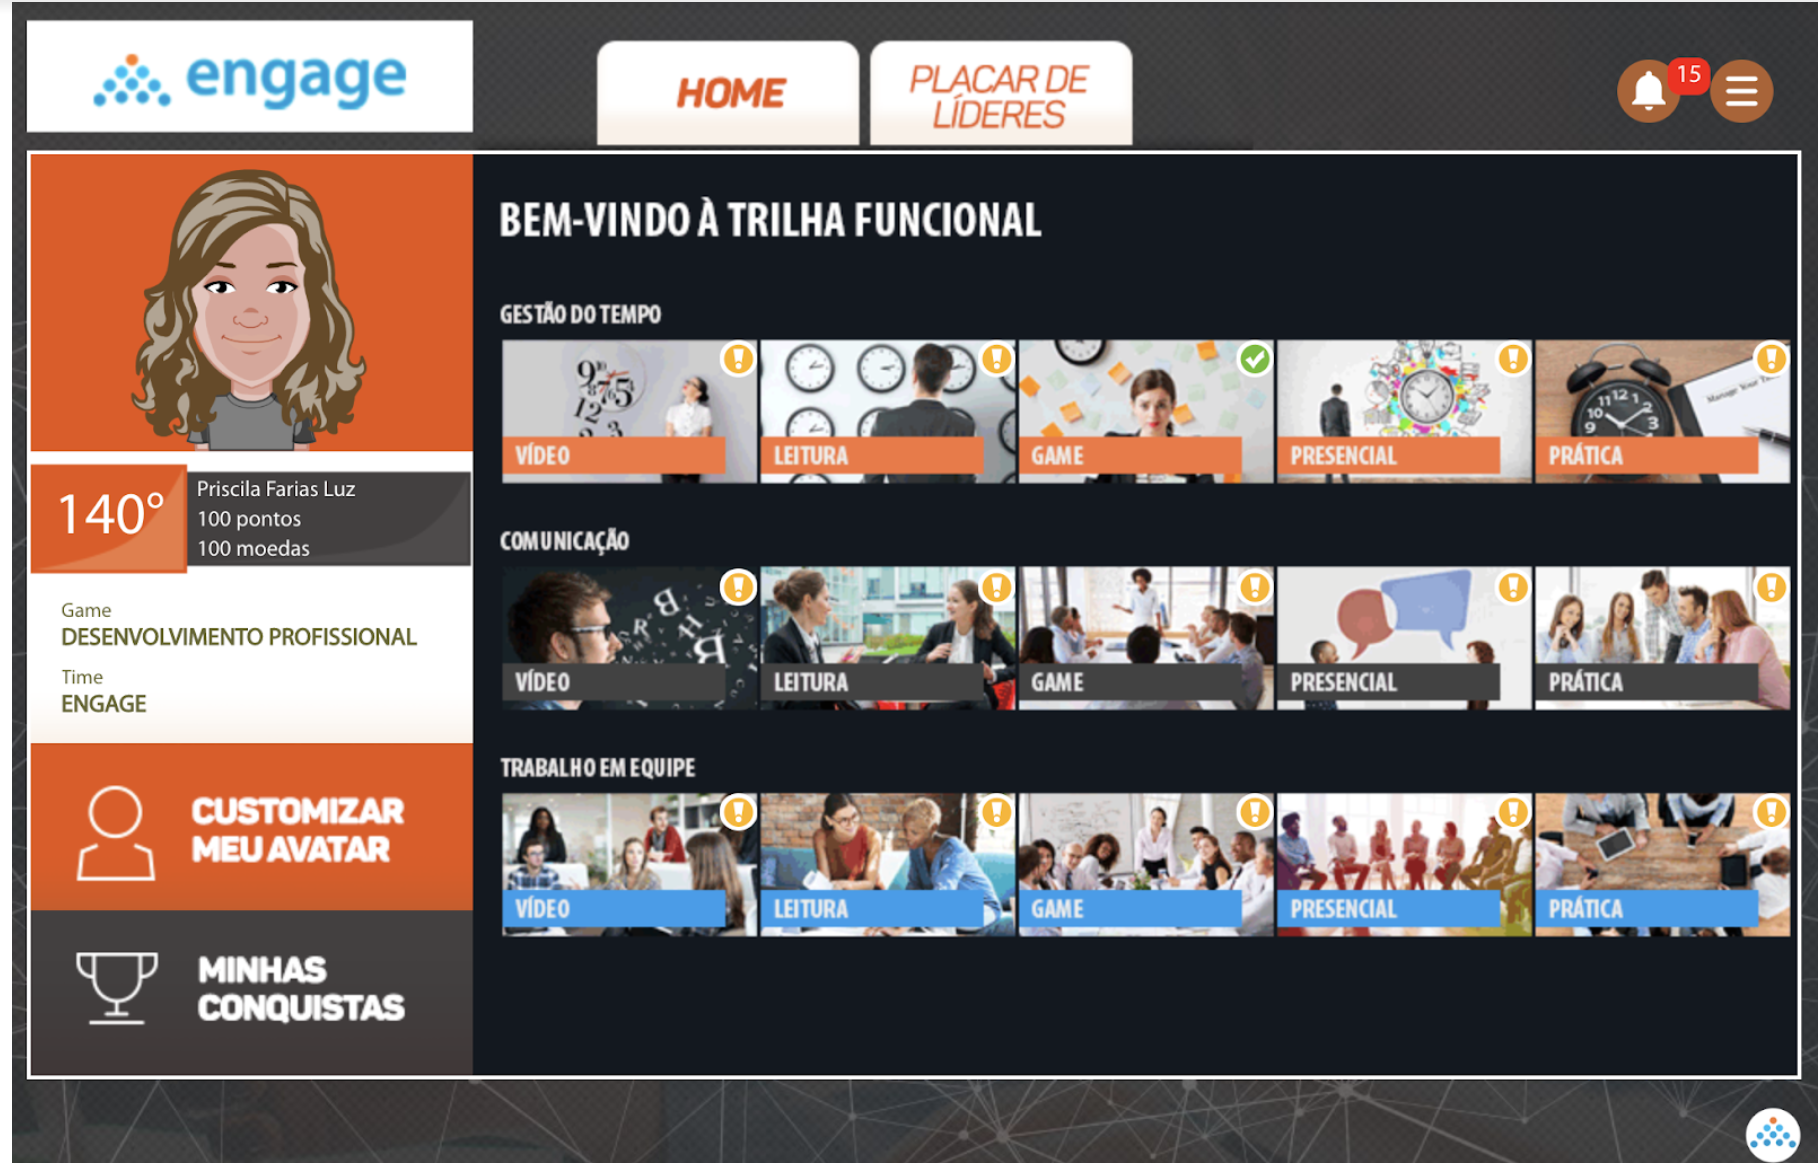
\includegraphics[width=15cm]{images/trabalhos-relacionados-img/img1-Engage.png}
  \caption{Exemplo da Plataforma Engage}
  \label{fig:exampleEngage}
\end{center}
\end{figure}


\section{Apta}

Ao acessar https://aptacursos.com.br  o usuário já encontrará a proposta do site que é "ser um ambiente de aprendizagem gamificado que promove informações inovadoras em áreas técnicas e profissionais, através de cursos onlines".

Nessa plataforma só tem permissão de criar novos cursos os proprietário criadores da mesma, porém um usuário pode requisitar a criação de um curso, para isso ele deve entrar em contato através do email ou telefone disponível na plataforma. Porém, é necessário destacar que essa é uma plataforma paga, ou seja, existe um custo associado à criação de um novo curso.

Como já foi dito, a Apta também utiliza alguns dos conceitos dos games na criação de seus cursos, a seguir serão enumerados alguns deles:

\begin{itemize}
\item A plataforma transforma cada curso é uma missão composta por uma série de desafios
\item Os desafios são de natureza diversa e podem incluir mini-jogos, quizzes, hipertextos, vídeos
\item A plataforma define metas a serem alcançadas pelos usuários do curso
\item Os alunos podem monitorar seu andamento através de ferramentas de avaliações
\end{itemize}

\begin{figure}[htp]
\begin{center}
  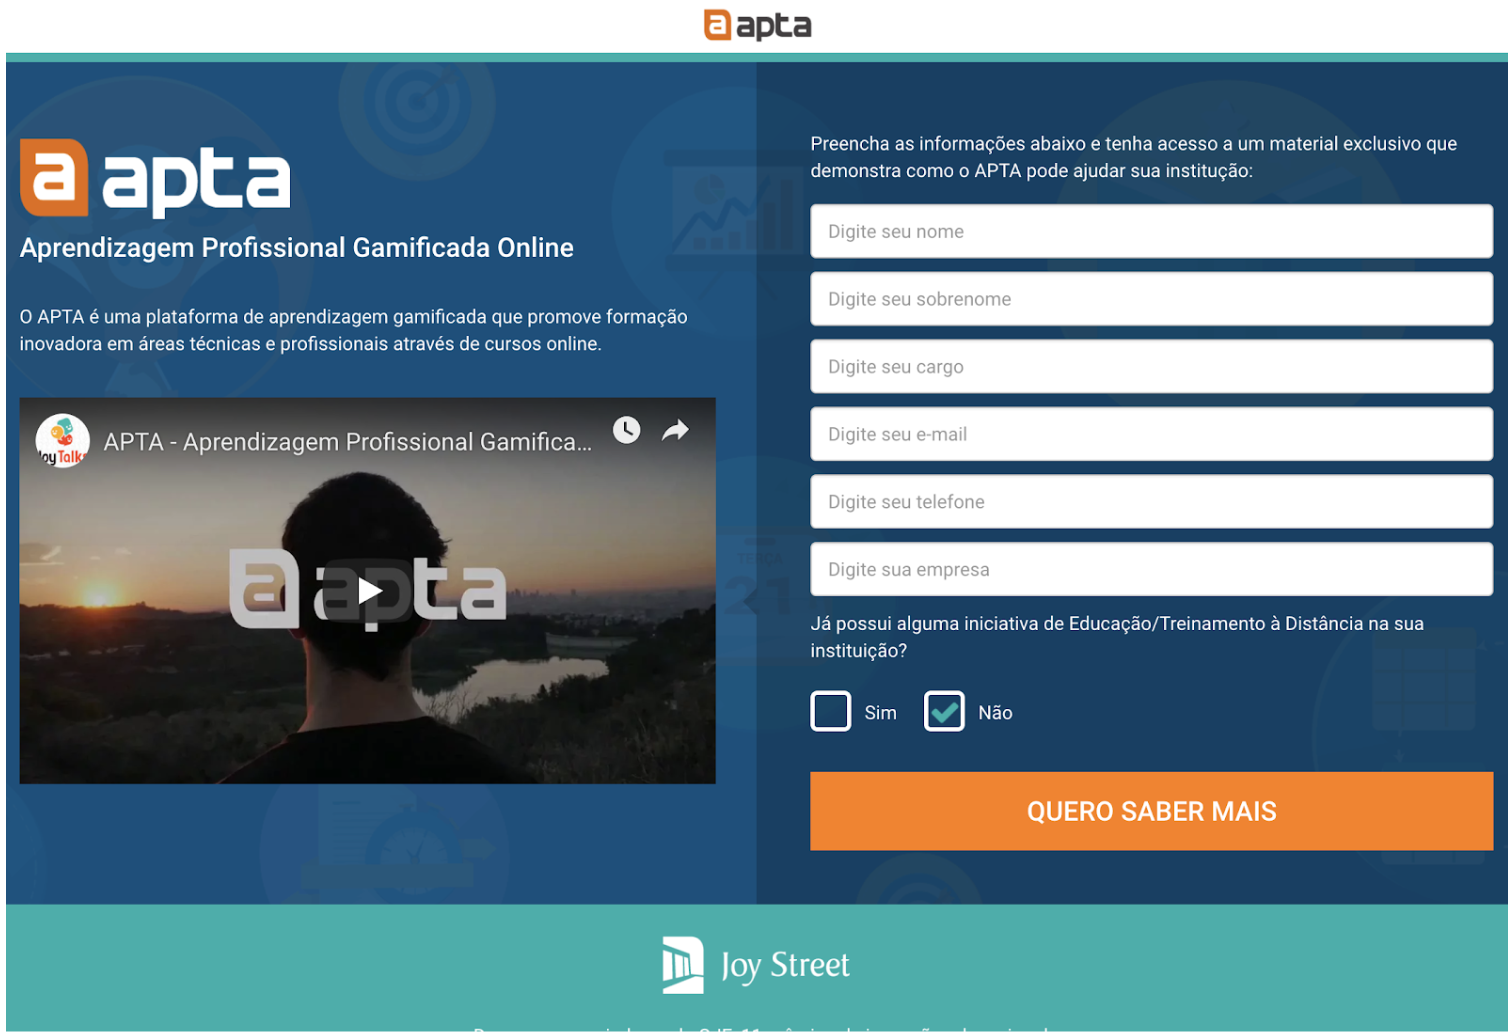
\includegraphics[width=12cm]{images/trabalhos-relacionados-img/img2-Apta.png}
  \caption{Exemplo da Plataforma Apta}
  \label{fig:exampleApta}
\end{center}
\end{figure}


\section{Moodle}

O moodle (Modular Object-Oriented Dynamic Learning Environment) é um software livre, que permite a criação de cursos, grupos de trabalho, páginas de disciplinas e comunidades. A primeira versão deste software foi disponibilizada em 2002 por seu criador Martin Dougiama, inicialmente ela foi criada para ser utilizada em faculdades, porém com o tempo ela invadiu outros ambiente como escolas e trabalho. Em questões de meses a plataforma ganhou o mundo e atualmente detém o título de ser a LMS mais popular que existe com 80 milhões de usuários em 222 territórios em todo o mundo. 

Algumas das funcionalidades existentes dentro dessa poderosa ferramenta são:

\begin{itemize}
\item Criações de cursos
\item Questionários
\item Avaliação dos professores
\item Criar comunidades em que os participantes possam se comunicar
\item Possibilidade do aluno de acompanhar suas próprias atividades
\end{itemize}

Como já foi mencionado, essa é uma poderosa ferramenta para ensino de conteúdo online, porém, um ponto negativo é que ela só permite ao professor criar cursos tradicionais, sem o uso de recursos visuais ou conceitos da gamificação.

\begin{figure}[htp]
\begin{center}
  
\includegraphics[width=10cm]{images/trabalhos-relacionados-img/img3-Moodle.png}
  \caption{Exemplo da Plataforma Moodle}
  \label{fig:exampleMoodle}
\end{center}
\end{figure}



\section{Kaptiva}

Mais uma plataforma de ensino que utiliza a gamificação nos seus cursos é kaptiva, esse ambiente de aprendizagem pode ser acessada através do link kaptiva.com.br.

Em sua página na Web ela demonstra ter como objetivo ser um "moodle gamificado". No tópico anterior já apresentamos a plataforma moodle e suas propostas, a diferencial da Kaptiva com relação ao moodle são basicamente três, a primeiro é o uso da gamificação feita por essa plataforma, algo que o moodle não se propõe a fazer, a segunda é ter como público alvo apenas empresas e por fim, temos a terceira que é o fato dessa plataforma ser paga diferente do moodle que como relatamos pode ser utilizado em diferentes ambiente de forma gratuita.

\begin{figure}[htp]
\begin{center}
  
\includegraphics[width=15cm]{images/trabalhos-relacionados-img/img4-Kaptiva.png}
  \caption{Exemplo da Plataforma Kaptiva}
  \label{fig:exampleKaptiva}
\end{center}
\end{figure}

\section{Dokeos}

O Dokeos, assim como o moodle, é uma LMS que não utiliza a gamificação, nessa plataforma, os professores podem criar cursos onlines para disponibilizar a um grupo de alunos, após os alunos começarem a utilizar o professor tem a opção de acompanhar o andamento de cada participante.

Esse ambiente de aprendizagem pode ser acessada através do link www.dokeos.com, além disso é site multiplataforma e tem a desvantagem de ser paga.

\begin{figure}[htp]
\begin{center}
  
\includegraphics[width=15cm]{images/trabalhos-relacionados-img/img5-Dokeos.png}
  \caption{Exemplo da Plataforma Dokeos}
  \label{fig:exampleDokeos}
\end{center}
\end{figure}


\chapter{Trabalhos Relacionados}
\label{ch:trabalhosRelacionados}

Existem diversas plataformas que utilizam a LMS e gamificação para ensinar algum conteúdo a um grupo. Muitas dessas páginas Webs contém algumas semelhanças com a GameInfor. Contudo, mesmo sabendo que todas essas plataformas  têm como objetivo explicar uma temática através de uma série de etapas, elas possuem algumas importantes diferenças na sua proposta, essas diferenças podem definir o público alvo, o interesse do aluno nos tópicos passados e o custo benefício do uso de uma página específica.

Neste capítulo serão mostraremos algumas dessas plataformas, para cada uma delas apresentaremos as suas funcionalidades, o seu público alvo, seus pontos positivos e negativos. As plataformas que vamos abordar são: Engage, Apta, Moodle, Kaptiva e Dokeos.

\section{Engage}

A engage é uma plataforma de ensino que pode ser acessada através do link https://www.engage.bz, ela fornece ao usuário a possibilidade de criar uma série de cursos sobre os mais diversos conteúdos. Esta plataforma tem como público alvo as empresas que desejam fornecer aos seus funcionários cursos diversos. A ideia da mesma é que a empresas façam uso de seus recursos para passar os conhecimentos aos empregados.

Está é uma plataforma gamificada, ou seja, ela utiliza conceitos de jogos para tornar o conteúdo mais atraente aos funcionários que participarão do curso. Alguns dos conceitos utilizados são:

\begin{itemize}
\item Jogo de perguntas: nesses jogos são utilizadas animações para atrair visualmente o usuário, um relógio de pontos, nessa funcionalidade o usuário terá uma pontuação máxima para responder a pergunta, a medida que o tempo passar os pontos que serão recebidos caso a pergunta seja respondida de forma correta vai diminuindo.
\item Ranking: com essa funcionalidade o usuário pode competir amigavelmente com seus colegas de trabalho, verificando quem está obtendo a melhor pontuação no curso.
\item Conquistas pessoais: além de acompanhar o ranking geral de todos que estão fazendo o curso, a pessoa também pode acompanhar seu próprio andamento.
\item Avatar: o indivíduo pode também criar avatar escolhendo características como sexo, cor da pele, cabelo, olho, boca e nariz.
\end{itemize}

Resumindo, essa é uma boa plataforma, porém ela tem como desvantagem o fato de ser paga e ter um escopo de usuários limitada.

\begin{figure}[htp]
\begin{center}
  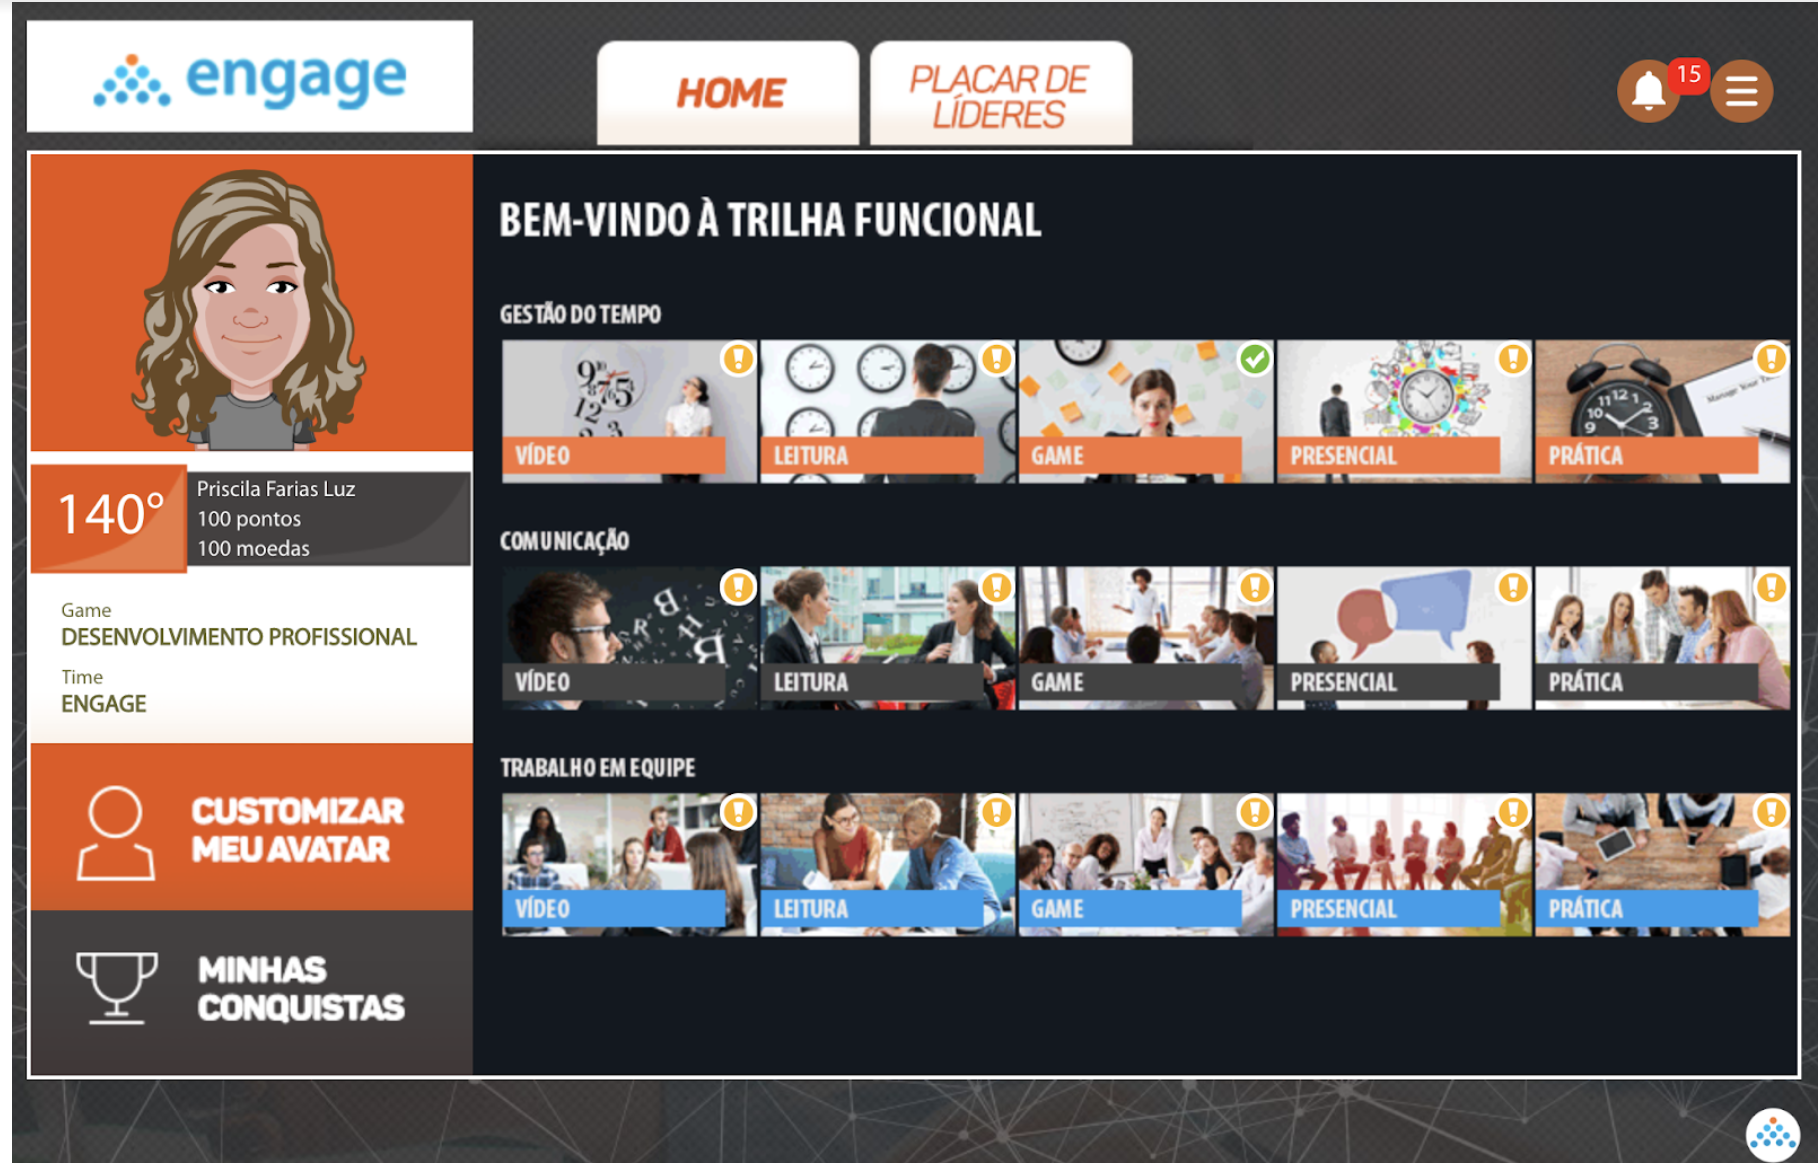
\includegraphics[width=15cm]{images/trabalhos-relacionados-img/img1-Engage.png}
  \caption{Exemplo da Plataforma Engage}
  \label{fig:exampleEngage}
\end{center}
\end{figure}


\section{Apta}

Ao acessar https://aptacursos.com.br  o usuário já encontrará a proposta do site que é "ser um ambiente de aprendizagem gamificado que promove informações inovadoras em áreas técnicas e profissionais, através de cursos onlines".

Nessa plataforma só tem permissão de criar novos cursos os proprietário criadores da mesma, porém um usuário pode requisitar a criação de um curso, para isso ele deve entrar em contato através do email ou telefone disponível na plataforma. Porém, é necessário destacar que essa é uma plataforma paga, ou seja, existe um custo associado à criação de um novo curso.

Como já foi dito, a Apta também utiliza alguns dos conceitos dos games na criação de seus cursos, a seguir serão enumerados alguns deles:

\begin{itemize}
\item A plataforma transforma cada curso é uma missão composta por uma série de desafios
\item Os desafios são de natureza diversa e podem incluir mini-jogos, quizzes, hipertextos, vídeos
\item A plataforma define metas a serem alcançadas pelos usuários do curso
\item Os alunos podem monitorar seu andamento através de ferramentas de avaliações
\end{itemize}

\begin{figure}[htp]
\begin{center}
  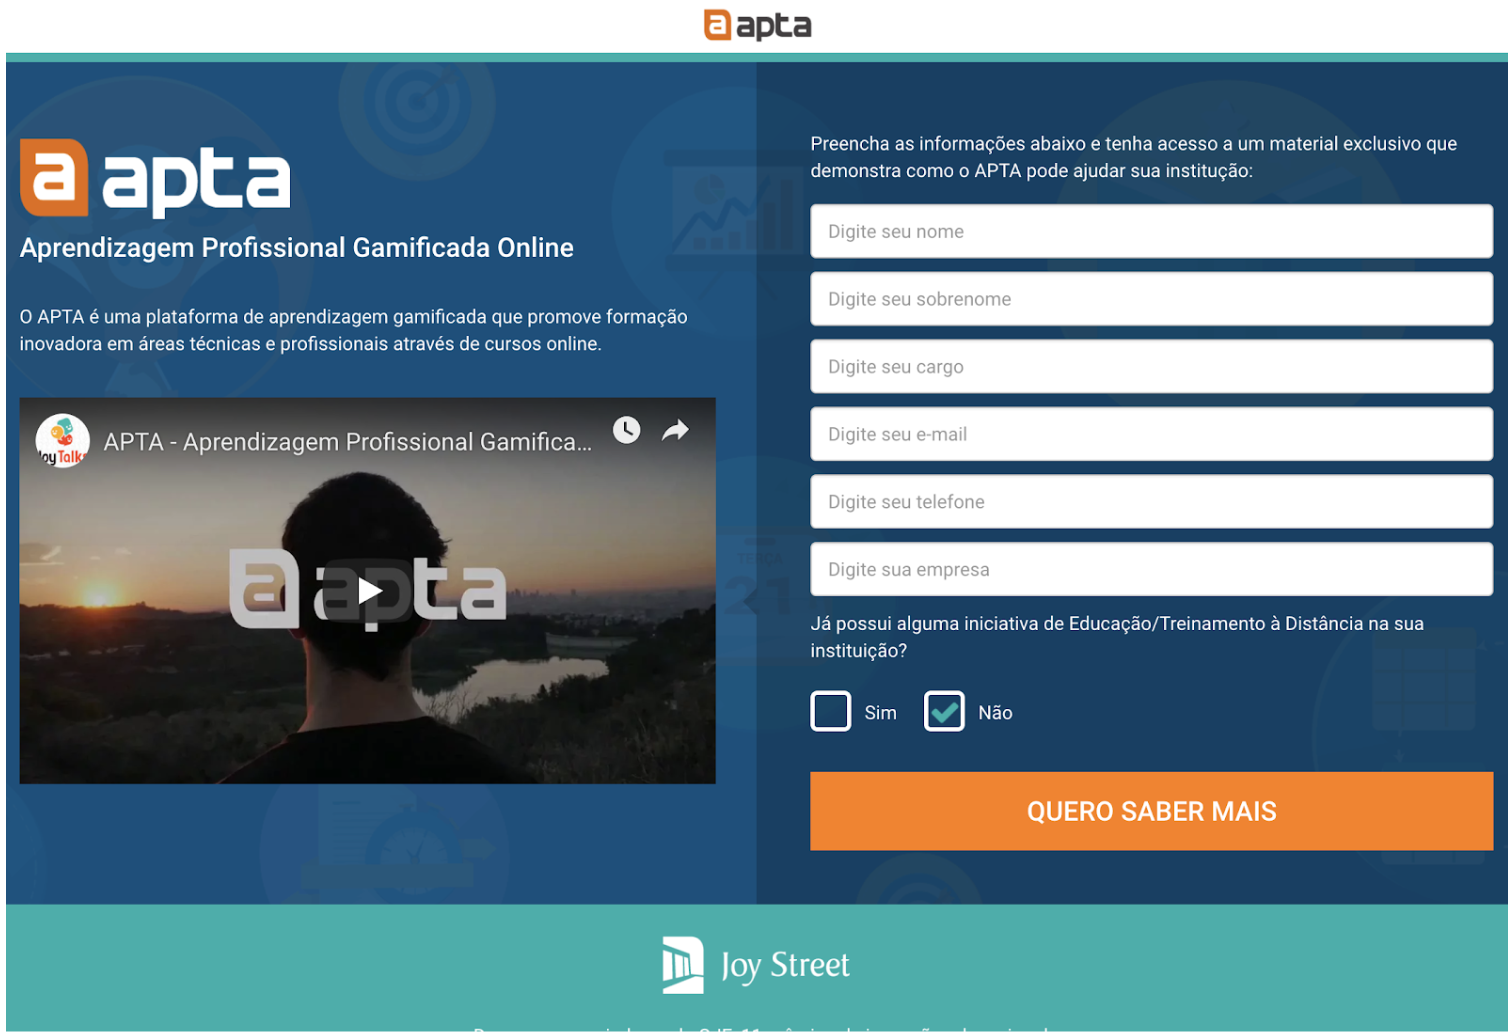
\includegraphics[width=12cm]{images/trabalhos-relacionados-img/img2-Apta.png}
  \caption{Exemplo da Plataforma Apta}
  \label{fig:exampleApta}
\end{center}
\end{figure}


\section{Moodle}

O moodle (Modular Object-Oriented Dynamic Learning Environment) é um software livre, que permite a criação de cursos, grupos de trabalho, páginas de disciplinas e comunidades. A primeira versão deste software foi disponibilizada em 2002 por seu criador Martin Dougiama, inicialmente ela foi criada para ser utilizada em faculdades, porém com o tempo ela invadiu outros ambiente como escolas e trabalho. Em questões de meses a plataforma ganhou o mundo e atualmente detém o título de ser a LMS mais popular que existe com 80 milhões de usuários em 222 territórios em todo o mundo. 

Algumas das funcionalidades existentes dentro dessa poderosa ferramenta são:

\begin{itemize}
\item Criações de cursos
\item Questionários
\item Avaliação dos professores
\item Criar comunidades em que os participantes possam se comunicar
\item Possibilidade do aluno de acompanhar suas próprias atividades
\end{itemize}

Como já foi mencionado, essa é uma poderosa ferramenta para ensino de conteúdo online, porém, um ponto negativo é que ela só permite ao professor criar cursos tradicionais, sem o uso de recursos visuais ou conceitos da gamificação.

\begin{figure}[htp]
\begin{center}
  
\includegraphics[width=10cm]{images/trabalhos-relacionados-img/img3-Moodle.png}
  \caption{Exemplo da Plataforma Moodle}
  \label{fig:exampleMoodle}
\end{center}
\end{figure}



\section{Kaptiva}

Mais uma plataforma de ensino que utiliza a gamificação nos seus cursos é kaptiva, esse ambiente de aprendizagem pode ser acessada através do link kaptiva.com.br.

Em sua página na Web ela demonstra ter como objetivo ser um "moodle gamificado". No tópico anterior já apresentamos a plataforma moodle e suas propostas, a diferencial da Kaptiva com relação ao moodle são basicamente três, a primeiro é o uso da gamificação feita por essa plataforma, algo que o moodle não se propõe a fazer, a segunda é ter como público alvo apenas empresas e por fim, temos a terceira que é o fato dessa plataforma ser paga diferente do moodle que como relatamos pode ser utilizado em diferentes ambiente de forma gratuita.

\begin{figure}[htp]
\begin{center}
  
\includegraphics[width=15cm]{images/trabalhos-relacionados-img/img4-Kaptiva.png}
  \caption{Exemplo da Plataforma Kaptiva}
  \label{fig:exampleKaptiva}
\end{center}
\end{figure}

\section{Dokeos}

O Dokeos, assim como o moodle, é uma LMS que não utiliza a gamificação, nessa plataforma, os professores podem criar cursos onlines para disponibilizar a um grupo de alunos, após os alunos começarem a utilizar o professor tem a opção de acompanhar o andamento de cada participante.

Esse ambiente de aprendizagem pode ser acessada através do link www.dokeos.com, além disso é site multiplataforma e tem a desvantagem de ser paga.

\begin{figure}[htp]
\begin{center}
  
\includegraphics[width=15cm]{images/trabalhos-relacionados-img/img5-Dokeos.png}
  \caption{Exemplo da Plataforma Dokeos}
  \label{fig:exampleDokeos}
\end{center}
\end{figure}


\chapter{Trabalhos Relacionados}
\label{ch:trabalhosRelacionados}

Existem diversas plataformas que utilizam a LMS e gamificação para ensinar algum conteúdo a um grupo. Muitas dessas páginas Webs contém algumas semelhanças com a GameInfor. Contudo, mesmo sabendo que todas essas plataformas  têm como objetivo explicar uma temática através de uma série de etapas, elas possuem algumas importantes diferenças na sua proposta, essas diferenças podem definir o público alvo, o interesse do aluno nos tópicos passados e o custo benefício do uso de uma página específica.

Neste capítulo serão mostraremos algumas dessas plataformas, para cada uma delas apresentaremos as suas funcionalidades, o seu público alvo, seus pontos positivos e negativos. As plataformas que vamos abordar são: Engage, Apta, Moodle, Kaptiva e Dokeos.

\section{Engage}

A engage é uma plataforma de ensino que pode ser acessada através do link https://www.engage.bz, ela fornece ao usuário a possibilidade de criar uma série de cursos sobre os mais diversos conteúdos. Esta plataforma tem como público alvo as empresas que desejam fornecer aos seus funcionários cursos diversos. A ideia da mesma é que a empresas façam uso de seus recursos para passar os conhecimentos aos empregados.

Está é uma plataforma gamificada, ou seja, ela utiliza conceitos de jogos para tornar o conteúdo mais atraente aos funcionários que participarão do curso. Alguns dos conceitos utilizados são:

\begin{itemize}
\item Jogo de perguntas: nesses jogos são utilizadas animações para atrair visualmente o usuário, um relógio de pontos, nessa funcionalidade o usuário terá uma pontuação máxima para responder a pergunta, a medida que o tempo passar os pontos que serão recebidos caso a pergunta seja respondida de forma correta vai diminuindo.
\item Ranking: com essa funcionalidade o usuário pode competir amigavelmente com seus colegas de trabalho, verificando quem está obtendo a melhor pontuação no curso.
\item Conquistas pessoais: além de acompanhar o ranking geral de todos que estão fazendo o curso, a pessoa também pode acompanhar seu próprio andamento.
\item Avatar: o indivíduo pode também criar avatar escolhendo características como sexo, cor da pele, cabelo, olho, boca e nariz.
\end{itemize}

Resumindo, essa é uma boa plataforma, porém ela tem como desvantagem o fato de ser paga e ter um escopo de usuários limitada.

\begin{figure}[htp]
\begin{center}
  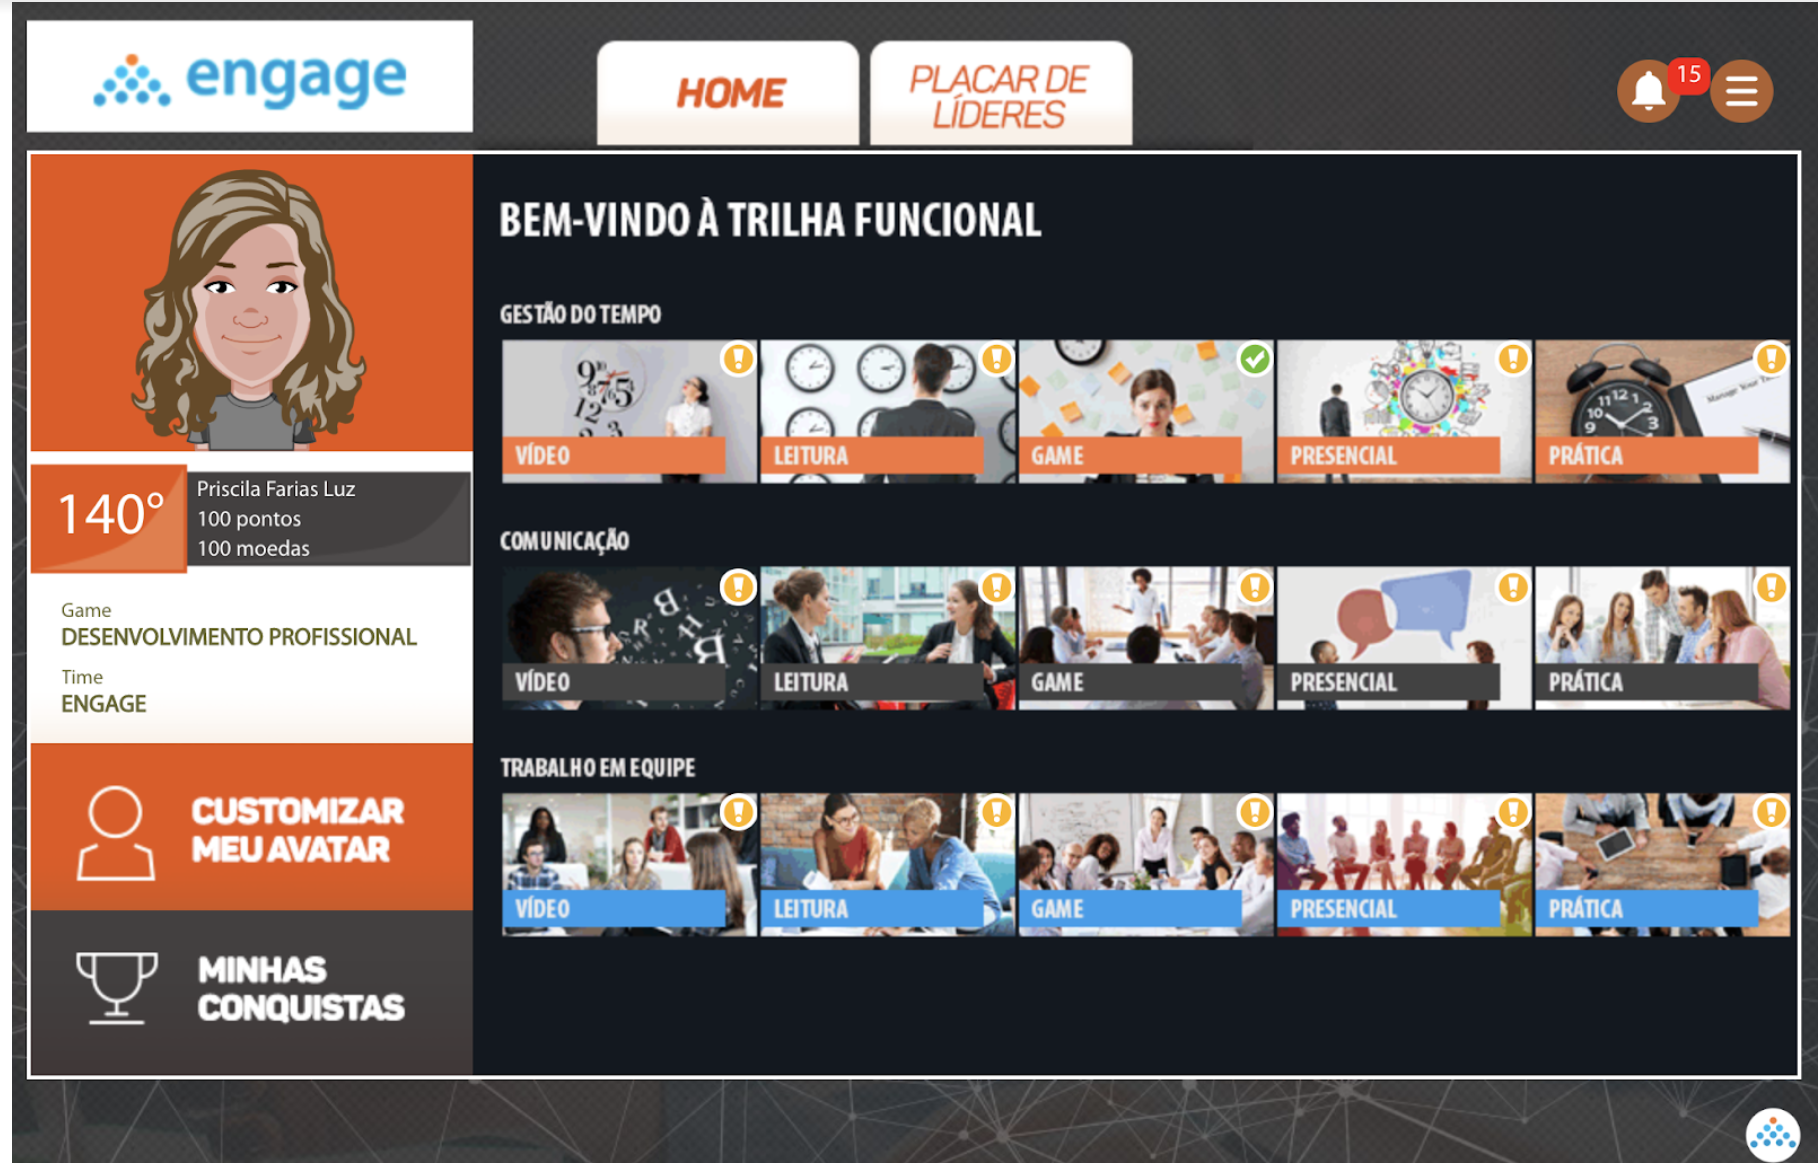
\includegraphics[width=15cm]{images/trabalhos-relacionados-img/img1-Engage.png}
  \caption{Exemplo da Plataforma Engage}
  \label{fig:exampleEngage}
\end{center}
\end{figure}


\section{Apta}

Ao acessar https://aptacursos.com.br  o usuário já encontrará a proposta do site que é "ser um ambiente de aprendizagem gamificado que promove informações inovadoras em áreas técnicas e profissionais, através de cursos onlines".

Nessa plataforma só tem permissão de criar novos cursos os proprietário criadores da mesma, porém um usuário pode requisitar a criação de um curso, para isso ele deve entrar em contato através do email ou telefone disponível na plataforma. Porém, é necessário destacar que essa é uma plataforma paga, ou seja, existe um custo associado à criação de um novo curso.

Como já foi dito, a Apta também utiliza alguns dos conceitos dos games na criação de seus cursos, a seguir serão enumerados alguns deles:

\begin{itemize}
\item A plataforma transforma cada curso é uma missão composta por uma série de desafios
\item Os desafios são de natureza diversa e podem incluir mini-jogos, quizzes, hipertextos, vídeos
\item A plataforma define metas a serem alcançadas pelos usuários do curso
\item Os alunos podem monitorar seu andamento através de ferramentas de avaliações
\end{itemize}

\begin{figure}[htp]
\begin{center}
  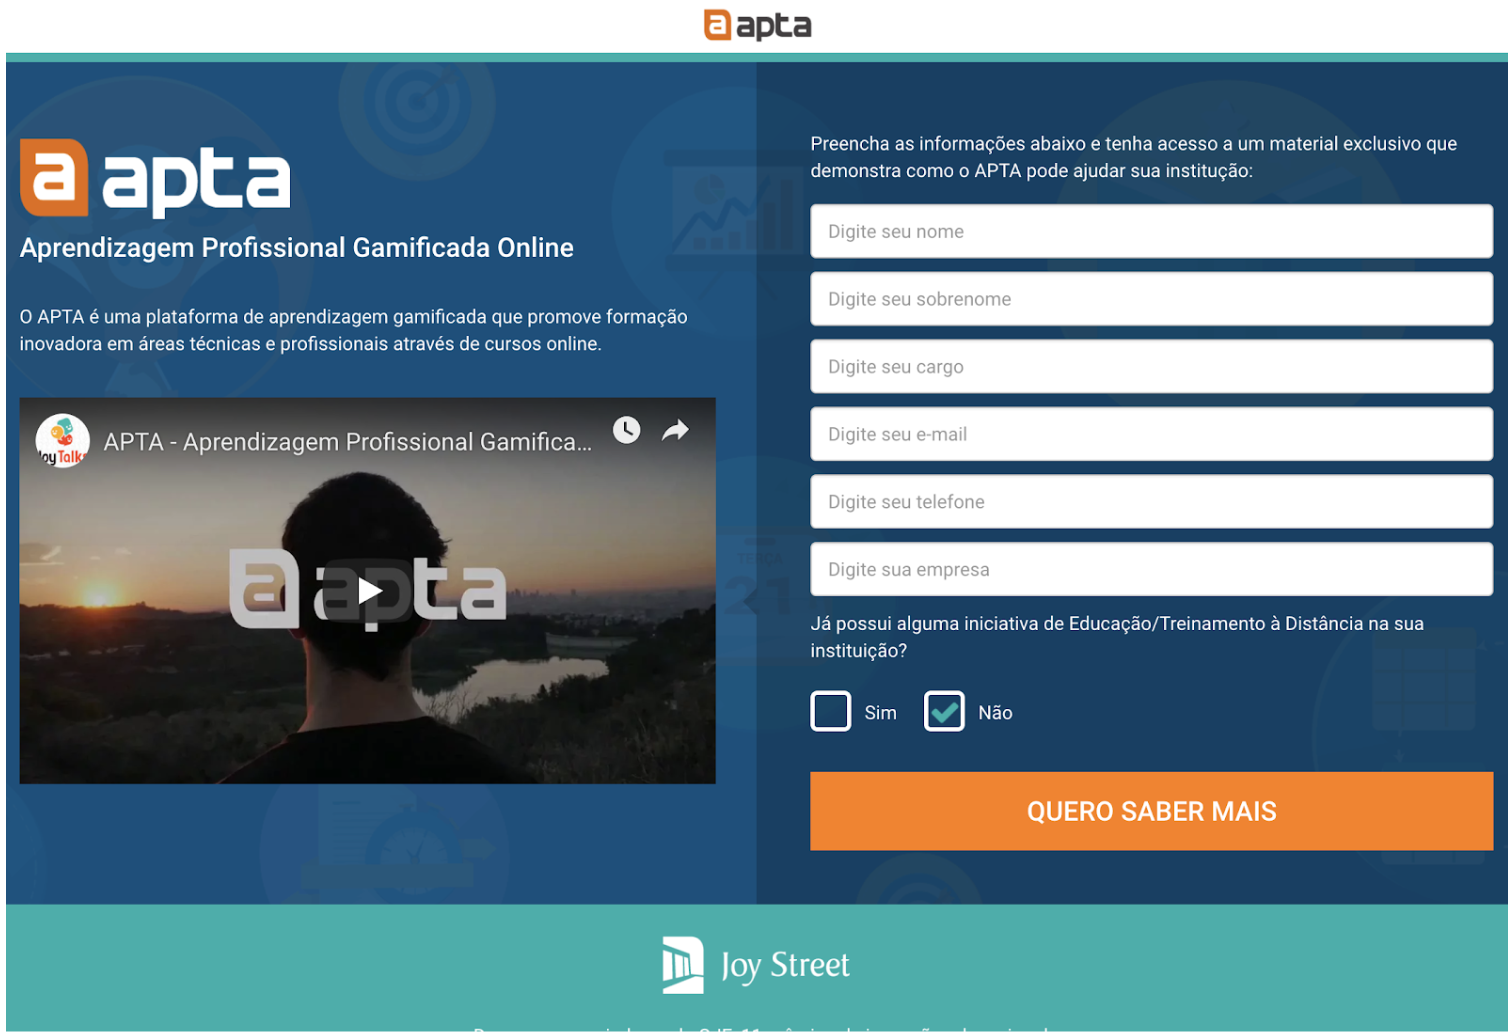
\includegraphics[width=12cm]{images/trabalhos-relacionados-img/img2-Apta.png}
  \caption{Exemplo da Plataforma Apta}
  \label{fig:exampleApta}
\end{center}
\end{figure}


\section{Moodle}

O moodle (Modular Object-Oriented Dynamic Learning Environment) é um software livre, que permite a criação de cursos, grupos de trabalho, páginas de disciplinas e comunidades. A primeira versão deste software foi disponibilizada em 2002 por seu criador Martin Dougiama, inicialmente ela foi criada para ser utilizada em faculdades, porém com o tempo ela invadiu outros ambiente como escolas e trabalho. Em questões de meses a plataforma ganhou o mundo e atualmente detém o título de ser a LMS mais popular que existe com 80 milhões de usuários em 222 territórios em todo o mundo. 

Algumas das funcionalidades existentes dentro dessa poderosa ferramenta são:

\begin{itemize}
\item Criações de cursos
\item Questionários
\item Avaliação dos professores
\item Criar comunidades em que os participantes possam se comunicar
\item Possibilidade do aluno de acompanhar suas próprias atividades
\end{itemize}

Como já foi mencionado, essa é uma poderosa ferramenta para ensino de conteúdo online, porém, um ponto negativo é que ela só permite ao professor criar cursos tradicionais, sem o uso de recursos visuais ou conceitos da gamificação.

\begin{figure}[htp]
\begin{center}
  
\includegraphics[width=10cm]{images/trabalhos-relacionados-img/img3-Moodle.png}
  \caption{Exemplo da Plataforma Moodle}
  \label{fig:exampleMoodle}
\end{center}
\end{figure}



\section{Kaptiva}

Mais uma plataforma de ensino que utiliza a gamificação nos seus cursos é kaptiva, esse ambiente de aprendizagem pode ser acessada através do link kaptiva.com.br.

Em sua página na Web ela demonstra ter como objetivo ser um "moodle gamificado". No tópico anterior já apresentamos a plataforma moodle e suas propostas, a diferencial da Kaptiva com relação ao moodle são basicamente três, a primeiro é o uso da gamificação feita por essa plataforma, algo que o moodle não se propõe a fazer, a segunda é ter como público alvo apenas empresas e por fim, temos a terceira que é o fato dessa plataforma ser paga diferente do moodle que como relatamos pode ser utilizado em diferentes ambiente de forma gratuita.

\begin{figure}[htp]
\begin{center}
  
\includegraphics[width=15cm]{images/trabalhos-relacionados-img/img4-Kaptiva.png}
  \caption{Exemplo da Plataforma Kaptiva}
  \label{fig:exampleKaptiva}
\end{center}
\end{figure}

\section{Dokeos}

O Dokeos, assim como o moodle, é uma LMS que não utiliza a gamificação, nessa plataforma, os professores podem criar cursos onlines para disponibilizar a um grupo de alunos, após os alunos começarem a utilizar o professor tem a opção de acompanhar o andamento de cada participante.

Esse ambiente de aprendizagem pode ser acessada através do link www.dokeos.com, além disso é site multiplataforma e tem a desvantagem de ser paga.

\begin{figure}[htp]
\begin{center}
  
\includegraphics[width=15cm]{images/trabalhos-relacionados-img/img5-Dokeos.png}
  \caption{Exemplo da Plataforma Dokeos}
  \label{fig:exampleDokeos}
\end{center}
\end{figure}


\chapter{Trabalhos Relacionados}
\label{ch:trabalhosRelacionados}

Existem diversas plataformas que utilizam a LMS e gamificação para ensinar algum conteúdo a um grupo. Muitas dessas páginas Webs contém algumas semelhanças com a GameInfor. Contudo, mesmo sabendo que todas essas plataformas  têm como objetivo explicar uma temática através de uma série de etapas, elas possuem algumas importantes diferenças na sua proposta, essas diferenças podem definir o público alvo, o interesse do aluno nos tópicos passados e o custo benefício do uso de uma página específica.

Neste capítulo serão mostraremos algumas dessas plataformas, para cada uma delas apresentaremos as suas funcionalidades, o seu público alvo, seus pontos positivos e negativos. As plataformas que vamos abordar são: Engage, Apta, Moodle, Kaptiva e Dokeos.

\section{Engage}

A engage é uma plataforma de ensino que pode ser acessada através do link https://www.engage.bz, ela fornece ao usuário a possibilidade de criar uma série de cursos sobre os mais diversos conteúdos. Esta plataforma tem como público alvo as empresas que desejam fornecer aos seus funcionários cursos diversos. A ideia da mesma é que a empresas façam uso de seus recursos para passar os conhecimentos aos empregados.

Está é uma plataforma gamificada, ou seja, ela utiliza conceitos de jogos para tornar o conteúdo mais atraente aos funcionários que participarão do curso. Alguns dos conceitos utilizados são:

\begin{itemize}
\item Jogo de perguntas: nesses jogos são utilizadas animações para atrair visualmente o usuário, um relógio de pontos, nessa funcionalidade o usuário terá uma pontuação máxima para responder a pergunta, a medida que o tempo passar os pontos que serão recebidos caso a pergunta seja respondida de forma correta vai diminuindo.
\item Ranking: com essa funcionalidade o usuário pode competir amigavelmente com seus colegas de trabalho, verificando quem está obtendo a melhor pontuação no curso.
\item Conquistas pessoais: além de acompanhar o ranking geral de todos que estão fazendo o curso, a pessoa também pode acompanhar seu próprio andamento.
\item Avatar: o indivíduo pode também criar avatar escolhendo características como sexo, cor da pele, cabelo, olho, boca e nariz.
\end{itemize}

Resumindo, essa é uma boa plataforma, porém ela tem como desvantagem o fato de ser paga e ter um escopo de usuários limitada.

\begin{figure}[htp]
\begin{center}
  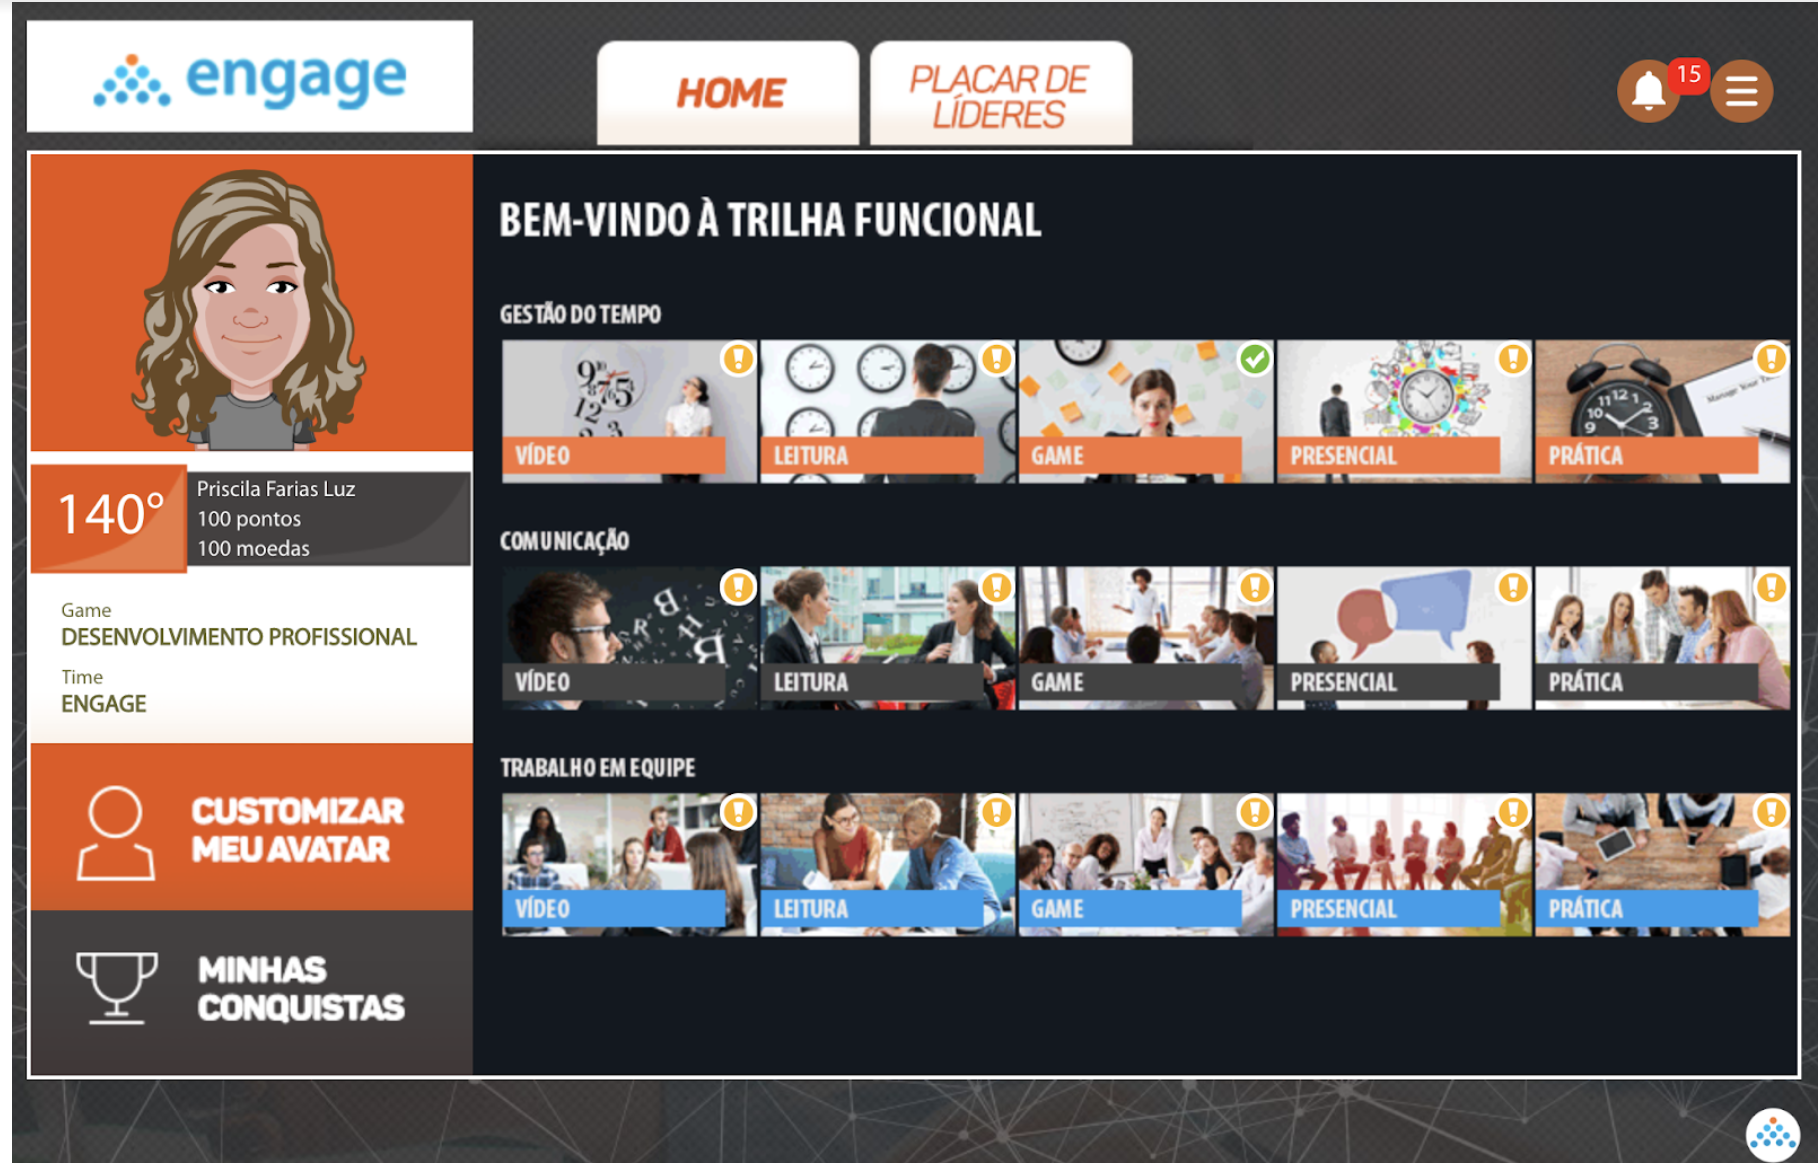
\includegraphics[width=15cm]{images/trabalhos-relacionados-img/img1-Engage.png}
  \caption{Exemplo da Plataforma Engage}
  \label{fig:exampleEngage}
\end{center}
\end{figure}


\section{Apta}

Ao acessar https://aptacursos.com.br  o usuário já encontrará a proposta do site que é "ser um ambiente de aprendizagem gamificado que promove informações inovadoras em áreas técnicas e profissionais, através de cursos onlines".

Nessa plataforma só tem permissão de criar novos cursos os proprietário criadores da mesma, porém um usuário pode requisitar a criação de um curso, para isso ele deve entrar em contato através do email ou telefone disponível na plataforma. Porém, é necessário destacar que essa é uma plataforma paga, ou seja, existe um custo associado à criação de um novo curso.

Como já foi dito, a Apta também utiliza alguns dos conceitos dos games na criação de seus cursos, a seguir serão enumerados alguns deles:

\begin{itemize}
\item A plataforma transforma cada curso é uma missão composta por uma série de desafios
\item Os desafios são de natureza diversa e podem incluir mini-jogos, quizzes, hipertextos, vídeos
\item A plataforma define metas a serem alcançadas pelos usuários do curso
\item Os alunos podem monitorar seu andamento através de ferramentas de avaliações
\end{itemize}

\begin{figure}[htp]
\begin{center}
  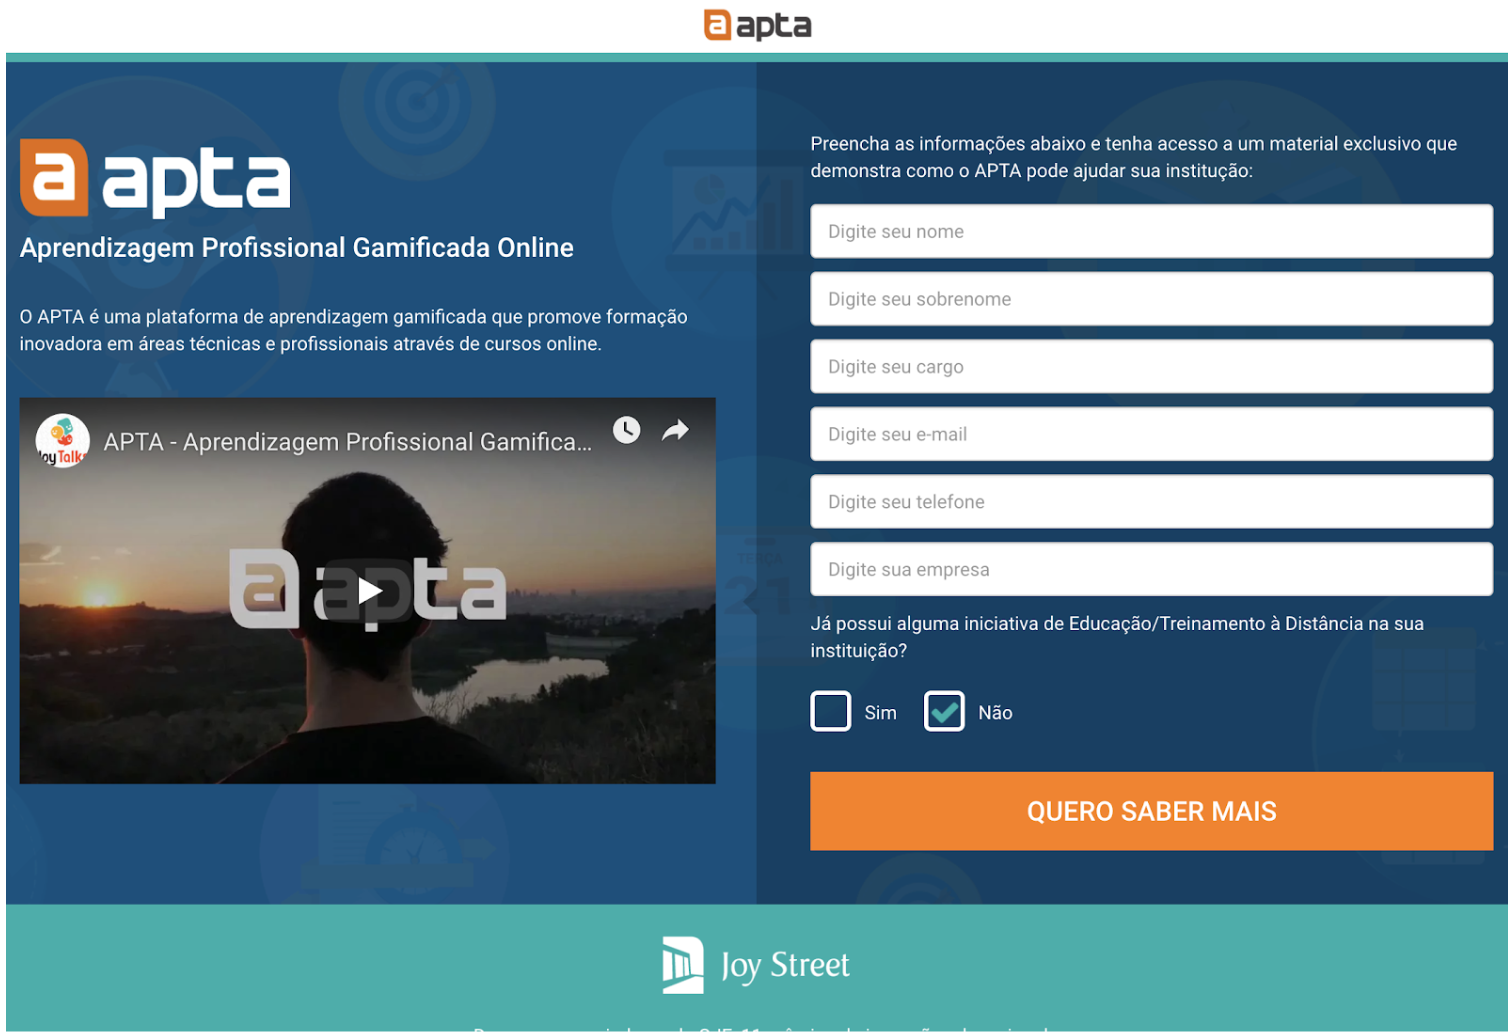
\includegraphics[width=12cm]{images/trabalhos-relacionados-img/img2-Apta.png}
  \caption{Exemplo da Plataforma Apta}
  \label{fig:exampleApta}
\end{center}
\end{figure}


\section{Moodle}

O moodle (Modular Object-Oriented Dynamic Learning Environment) é um software livre, que permite a criação de cursos, grupos de trabalho, páginas de disciplinas e comunidades. A primeira versão deste software foi disponibilizada em 2002 por seu criador Martin Dougiama, inicialmente ela foi criada para ser utilizada em faculdades, porém com o tempo ela invadiu outros ambiente como escolas e trabalho. Em questões de meses a plataforma ganhou o mundo e atualmente detém o título de ser a LMS mais popular que existe com 80 milhões de usuários em 222 territórios em todo o mundo. 

Algumas das funcionalidades existentes dentro dessa poderosa ferramenta são:

\begin{itemize}
\item Criações de cursos
\item Questionários
\item Avaliação dos professores
\item Criar comunidades em que os participantes possam se comunicar
\item Possibilidade do aluno de acompanhar suas próprias atividades
\end{itemize}

Como já foi mencionado, essa é uma poderosa ferramenta para ensino de conteúdo online, porém, um ponto negativo é que ela só permite ao professor criar cursos tradicionais, sem o uso de recursos visuais ou conceitos da gamificação.

\begin{figure}[htp]
\begin{center}
  
\includegraphics[width=10cm]{images/trabalhos-relacionados-img/img3-Moodle.png}
  \caption{Exemplo da Plataforma Moodle}
  \label{fig:exampleMoodle}
\end{center}
\end{figure}



\section{Kaptiva}

Mais uma plataforma de ensino que utiliza a gamificação nos seus cursos é kaptiva, esse ambiente de aprendizagem pode ser acessada através do link kaptiva.com.br.

Em sua página na Web ela demonstra ter como objetivo ser um "moodle gamificado". No tópico anterior já apresentamos a plataforma moodle e suas propostas, a diferencial da Kaptiva com relação ao moodle são basicamente três, a primeiro é o uso da gamificação feita por essa plataforma, algo que o moodle não se propõe a fazer, a segunda é ter como público alvo apenas empresas e por fim, temos a terceira que é o fato dessa plataforma ser paga diferente do moodle que como relatamos pode ser utilizado em diferentes ambiente de forma gratuita.

\begin{figure}[htp]
\begin{center}
  
\includegraphics[width=15cm]{images/trabalhos-relacionados-img/img4-Kaptiva.png}
  \caption{Exemplo da Plataforma Kaptiva}
  \label{fig:exampleKaptiva}
\end{center}
\end{figure}

\section{Dokeos}

O Dokeos, assim como o moodle, é uma LMS que não utiliza a gamificação, nessa plataforma, os professores podem criar cursos onlines para disponibilizar a um grupo de alunos, após os alunos começarem a utilizar o professor tem a opção de acompanhar o andamento de cada participante.

Esse ambiente de aprendizagem pode ser acessada através do link www.dokeos.com, além disso é site multiplataforma e tem a desvantagem de ser paga.

\begin{figure}[htp]
\begin{center}
  
\includegraphics[width=15cm]{images/trabalhos-relacionados-img/img5-Dokeos.png}
  \caption{Exemplo da Plataforma Dokeos}
  \label{fig:exampleDokeos}
\end{center}
\end{figure}


\chapter{Trabalhos Relacionados}
\label{ch:trabalhosRelacionados}

Existem diversas plataformas que utilizam a LMS e gamificação para ensinar algum conteúdo a um grupo. Muitas dessas páginas Webs contém algumas semelhanças com a GameInfor. Contudo, mesmo sabendo que todas essas plataformas  têm como objetivo explicar uma temática através de uma série de etapas, elas possuem algumas importantes diferenças na sua proposta, essas diferenças podem definir o público alvo, o interesse do aluno nos tópicos passados e o custo benefício do uso de uma página específica.

Neste capítulo serão mostraremos algumas dessas plataformas, para cada uma delas apresentaremos as suas funcionalidades, o seu público alvo, seus pontos positivos e negativos. As plataformas que vamos abordar são: Engage, Apta, Moodle, Kaptiva e Dokeos.

\section{Engage}

A engage é uma plataforma de ensino que pode ser acessada através do link https://www.engage.bz, ela fornece ao usuário a possibilidade de criar uma série de cursos sobre os mais diversos conteúdos. Esta plataforma tem como público alvo as empresas que desejam fornecer aos seus funcionários cursos diversos. A ideia da mesma é que a empresas façam uso de seus recursos para passar os conhecimentos aos empregados.

Está é uma plataforma gamificada, ou seja, ela utiliza conceitos de jogos para tornar o conteúdo mais atraente aos funcionários que participarão do curso. Alguns dos conceitos utilizados são:

\begin{itemize}
\item Jogo de perguntas: nesses jogos são utilizadas animações para atrair visualmente o usuário, um relógio de pontos, nessa funcionalidade o usuário terá uma pontuação máxima para responder a pergunta, a medida que o tempo passar os pontos que serão recebidos caso a pergunta seja respondida de forma correta vai diminuindo.
\item Ranking: com essa funcionalidade o usuário pode competir amigavelmente com seus colegas de trabalho, verificando quem está obtendo a melhor pontuação no curso.
\item Conquistas pessoais: além de acompanhar o ranking geral de todos que estão fazendo o curso, a pessoa também pode acompanhar seu próprio andamento.
\item Avatar: o indivíduo pode também criar avatar escolhendo características como sexo, cor da pele, cabelo, olho, boca e nariz.
\end{itemize}

Resumindo, essa é uma boa plataforma, porém ela tem como desvantagem o fato de ser paga e ter um escopo de usuários limitada.

\begin{figure}[htp]
\begin{center}
  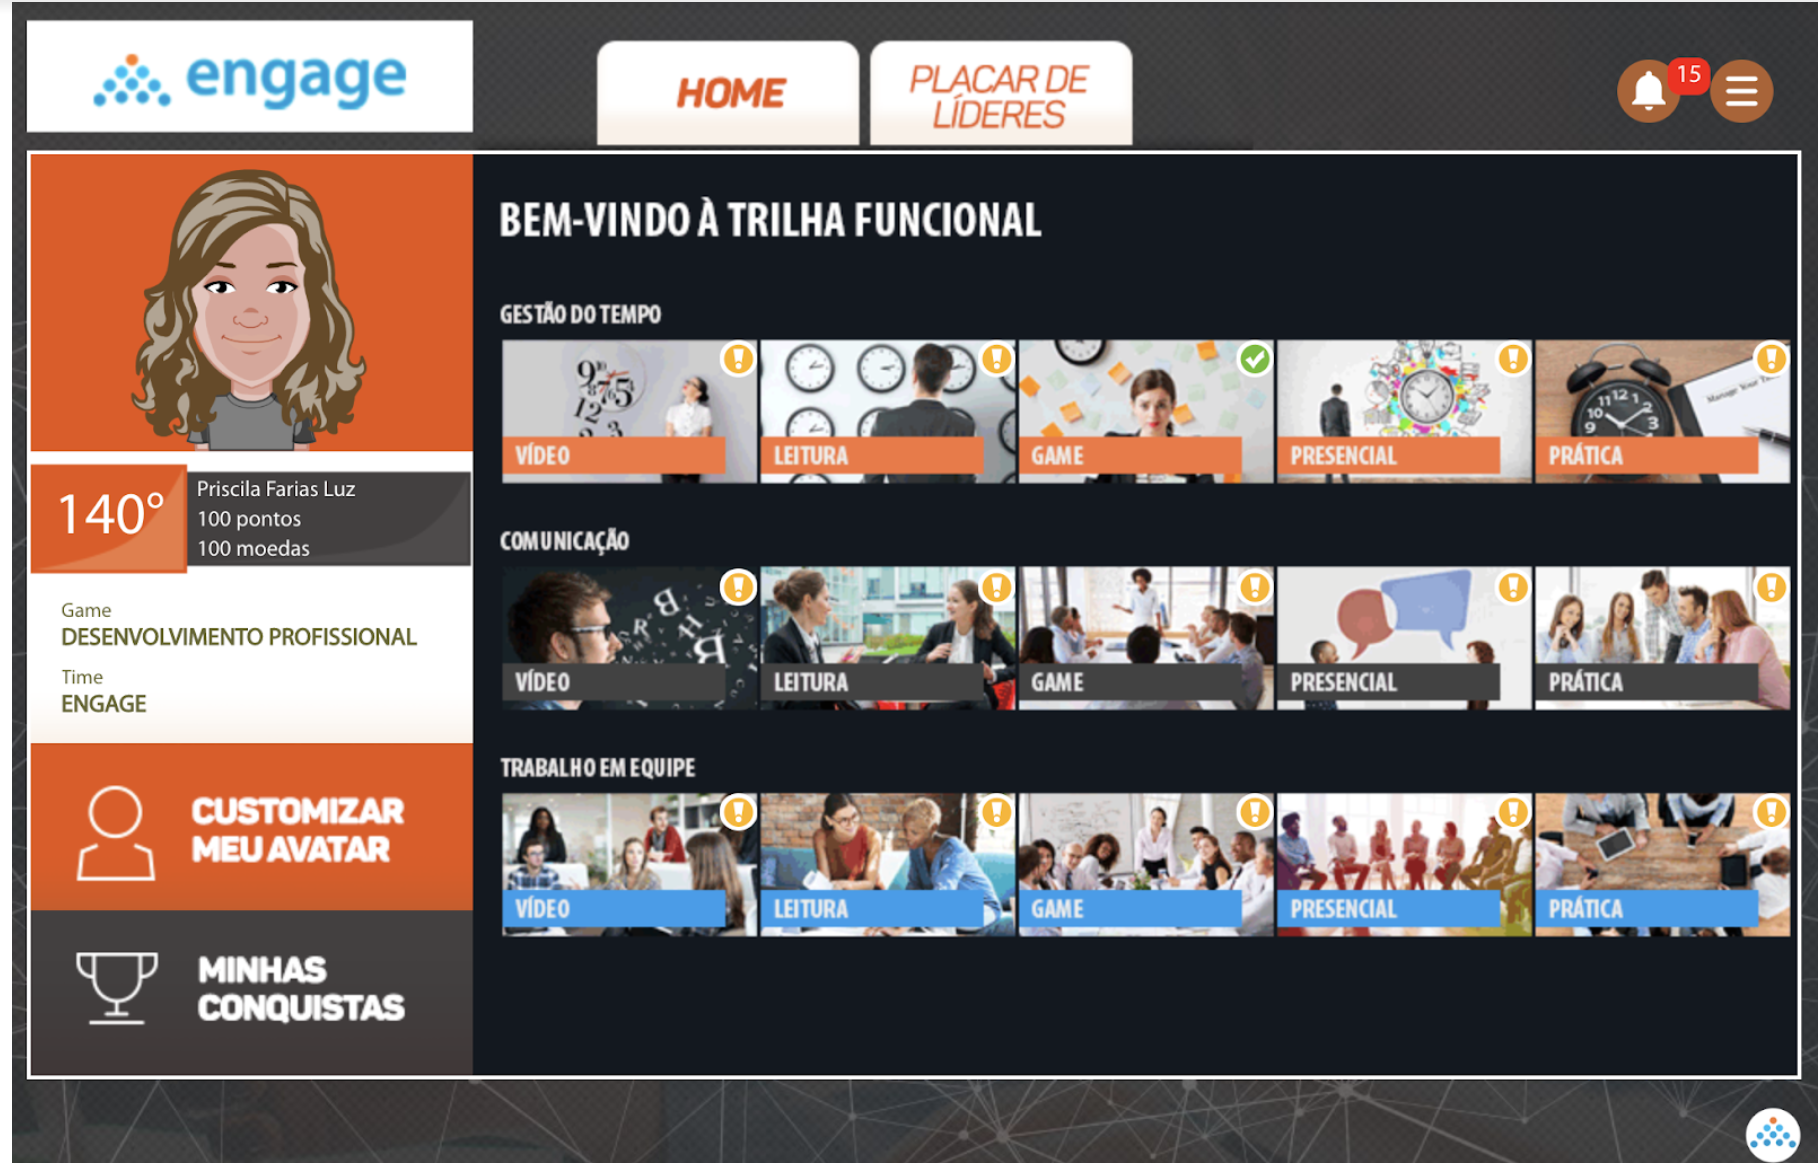
\includegraphics[width=15cm]{images/trabalhos-relacionados-img/img1-Engage.png}
  \caption{Exemplo da Plataforma Engage}
  \label{fig:exampleEngage}
\end{center}
\end{figure}


\section{Apta}

Ao acessar https://aptacursos.com.br  o usuário já encontrará a proposta do site que é "ser um ambiente de aprendizagem gamificado que promove informações inovadoras em áreas técnicas e profissionais, através de cursos onlines".

Nessa plataforma só tem permissão de criar novos cursos os proprietário criadores da mesma, porém um usuário pode requisitar a criação de um curso, para isso ele deve entrar em contato através do email ou telefone disponível na plataforma. Porém, é necessário destacar que essa é uma plataforma paga, ou seja, existe um custo associado à criação de um novo curso.

Como já foi dito, a Apta também utiliza alguns dos conceitos dos games na criação de seus cursos, a seguir serão enumerados alguns deles:

\begin{itemize}
\item A plataforma transforma cada curso é uma missão composta por uma série de desafios
\item Os desafios são de natureza diversa e podem incluir mini-jogos, quizzes, hipertextos, vídeos
\item A plataforma define metas a serem alcançadas pelos usuários do curso
\item Os alunos podem monitorar seu andamento através de ferramentas de avaliações
\end{itemize}

\begin{figure}[htp]
\begin{center}
  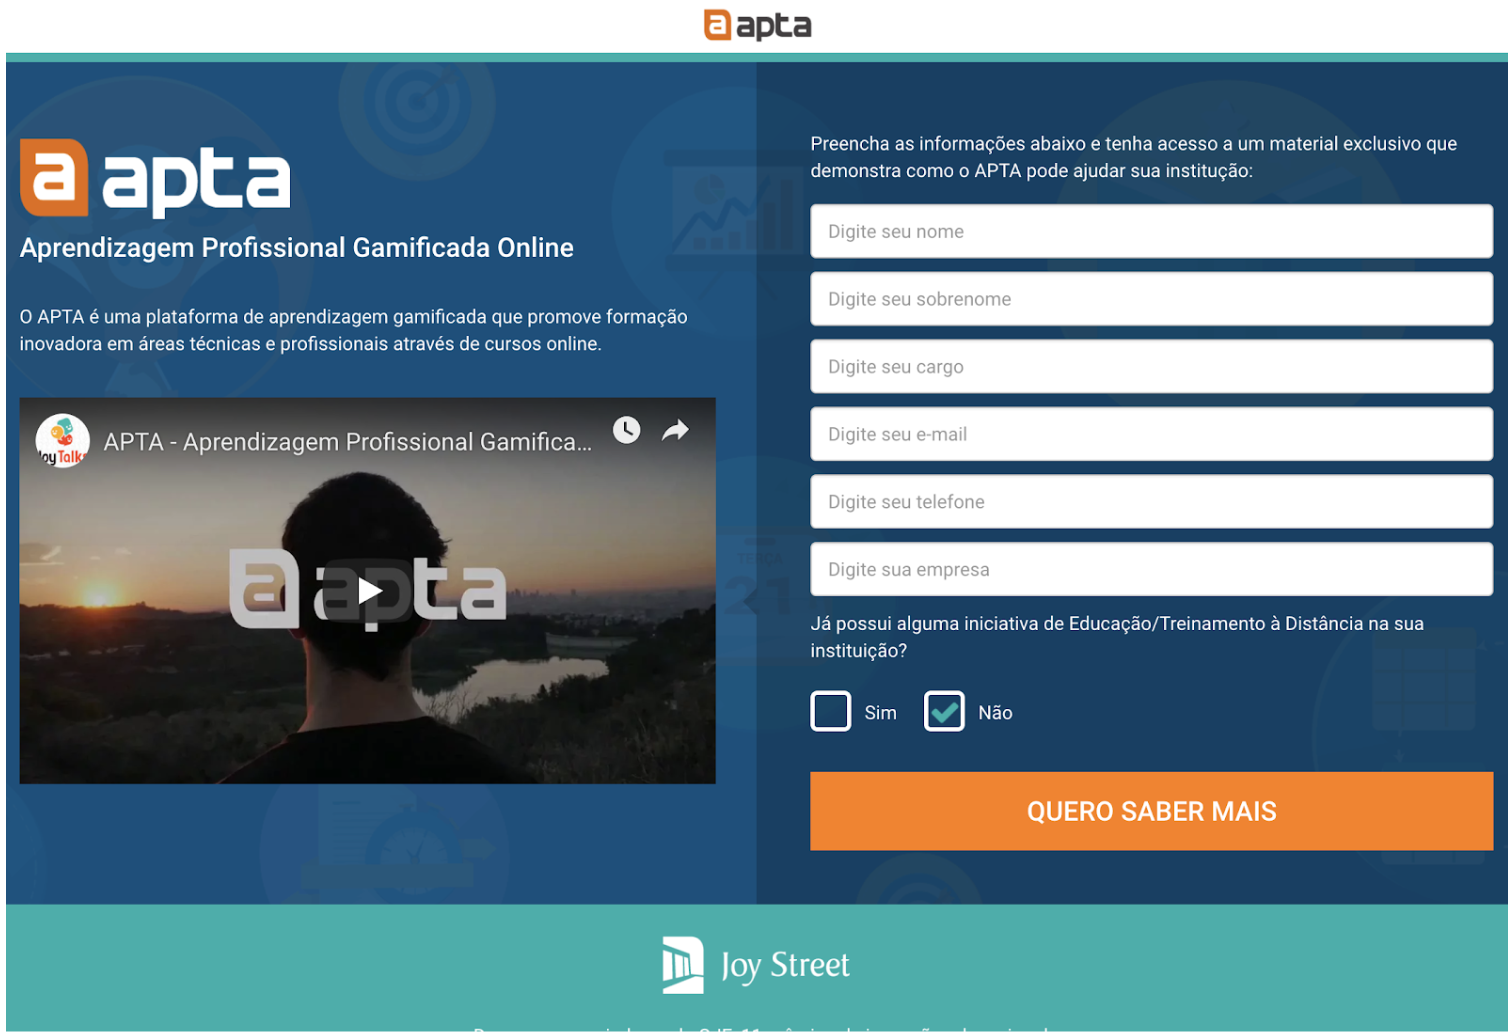
\includegraphics[width=12cm]{images/trabalhos-relacionados-img/img2-Apta.png}
  \caption{Exemplo da Plataforma Apta}
  \label{fig:exampleApta}
\end{center}
\end{figure}


\section{Moodle}

O moodle (Modular Object-Oriented Dynamic Learning Environment) é um software livre, que permite a criação de cursos, grupos de trabalho, páginas de disciplinas e comunidades. A primeira versão deste software foi disponibilizada em 2002 por seu criador Martin Dougiama, inicialmente ela foi criada para ser utilizada em faculdades, porém com o tempo ela invadiu outros ambiente como escolas e trabalho. Em questões de meses a plataforma ganhou o mundo e atualmente detém o título de ser a LMS mais popular que existe com 80 milhões de usuários em 222 territórios em todo o mundo. 

Algumas das funcionalidades existentes dentro dessa poderosa ferramenta são:

\begin{itemize}
\item Criações de cursos
\item Questionários
\item Avaliação dos professores
\item Criar comunidades em que os participantes possam se comunicar
\item Possibilidade do aluno de acompanhar suas próprias atividades
\end{itemize}

Como já foi mencionado, essa é uma poderosa ferramenta para ensino de conteúdo online, porém, um ponto negativo é que ela só permite ao professor criar cursos tradicionais, sem o uso de recursos visuais ou conceitos da gamificação.

\begin{figure}[htp]
\begin{center}
  
\includegraphics[width=10cm]{images/trabalhos-relacionados-img/img3-Moodle.png}
  \caption{Exemplo da Plataforma Moodle}
  \label{fig:exampleMoodle}
\end{center}
\end{figure}



\section{Kaptiva}

Mais uma plataforma de ensino que utiliza a gamificação nos seus cursos é kaptiva, esse ambiente de aprendizagem pode ser acessada através do link kaptiva.com.br.

Em sua página na Web ela demonstra ter como objetivo ser um "moodle gamificado". No tópico anterior já apresentamos a plataforma moodle e suas propostas, a diferencial da Kaptiva com relação ao moodle são basicamente três, a primeiro é o uso da gamificação feita por essa plataforma, algo que o moodle não se propõe a fazer, a segunda é ter como público alvo apenas empresas e por fim, temos a terceira que é o fato dessa plataforma ser paga diferente do moodle que como relatamos pode ser utilizado em diferentes ambiente de forma gratuita.

\begin{figure}[htp]
\begin{center}
  
\includegraphics[width=15cm]{images/trabalhos-relacionados-img/img4-Kaptiva.png}
  \caption{Exemplo da Plataforma Kaptiva}
  \label{fig:exampleKaptiva}
\end{center}
\end{figure}

\section{Dokeos}

O Dokeos, assim como o moodle, é uma LMS que não utiliza a gamificação, nessa plataforma, os professores podem criar cursos onlines para disponibilizar a um grupo de alunos, após os alunos começarem a utilizar o professor tem a opção de acompanhar o andamento de cada participante.

Esse ambiente de aprendizagem pode ser acessada através do link www.dokeos.com, além disso é site multiplataforma e tem a desvantagem de ser paga.

\begin{figure}[htp]
\begin{center}
  
\includegraphics[width=15cm]{images/trabalhos-relacionados-img/img5-Dokeos.png}
  \caption{Exemplo da Plataforma Dokeos}
  \label{fig:exampleDokeos}
\end{center}
\end{figure}




\bibliographystyle{natbib}
\addcontentsline{toc}{chapter}{\bibliographytocname}
\bibliography{references}

% Appendix
\clearpage
\addappheadtotoc
\appendix
\appendixpage
\chapter{Case Study Instruments}
\label{ap:measurement-instruments}


\def \tick{
$[$\hspace{0.3cm}$]$
}

\def \twooption#1#2{
\tick #1.  \tick #2.
}

\def \threeoption#1#2#3{
\tick #1.\newline
\tick #2.\newline
\tick #3.
}

\def \fouroption#1#2#3#4{
\tick #1.\newline
\tick #2.\newline
\tick #3.\newline
\tick #4.
}

\def \fiveoption#1#2#3#4#5{
\tick #1.\newline
\tick #2.\newline
\tick #3.\newline
\tick #4.\newline
\tick #5.
}
\def \datefield{
%date fied used in time sheets
    /\hspace{0.4cm}/
}

\def \rcolor{
%table row color
    \rowcolor[gray]{0.9}
}

\def \hcolor{
    \rowcolor[gray]{0.7}
}


\section{Form for Expert Survey}
\label{ap:sec:feedback}

\textbf{Name: }
\\
\line(1,0){380}
\\
\textbf{What is your experience with programming (in months/years) ? }
\\
\line(1,0){410}
\\
\line(1,0){410}
\\
\textbf{What is your experience with Software Product Lines ? }
\\
\line(1,0){410}
\\
\line(1,0){410}
\\
\textbf{There was any difficult during the execution of some activity in the tool ?}
\\
\twooption{Yes}{No}
\\
\textbf{In case you answered “Yes”,detail the difficulty encountered:}
\\
\line(1,0){410}
\\
\line(1,0){410}
\\
\line(1,0){410}
\\
\line(1,0){410}
\\
\textbf{How the usage of the tool altered your workflow ?  }
\\
\line(1,0){410}
\\
\line(1,0){410}
\\
\line(1,0){410}
\\
\line(1,0){410}
\\
\textbf{Did you have any problems creating assets ?}
\\
\twooption{Yes}{No}
\\
\textbf{In case you answered “Yes”,describe the problems encountered:}
\\
\line(1,0){410}
\\
\line(1,0){410}
\\
\line(1,0){410}
\\
\line(1,0){410}
\\
\textbf{Did the tool gave you enough information to identify who did a specific modification in an asset ?}
\\
\twooption{Yes}{No}
\\
\textbf{In case you answered “No”,describe what was missing:}
\\
\line(1,0){410}
\\
\line(1,0){410}
\\
\line(1,0){410}
\\
\line(1,0){410}
\\
\textbf{Do you consider that tool aided the traceability among the assets?}
\\
\twooption{Yes}{No}
\\
\textbf{Justify:}
\\
\line(1,0){410}
\\
\line(1,0){410}
\\
\line(1,0){410}
\\
\line(1,0){410}
\\
\textbf{Did you expect any traceability link not available in the tool ? If so, which one(s) ?}
\\
\line(1,0){410}
\\
\line(1,0){410}
\\
\line(1,0){410}
\\
\line(1,0){410}
\\
\textbf{What is your opinions on navigating among traceability links ?}
\\
\line(1,0){410}
\\
\line(1,0){410}
\\
\line(1,0){410}
\\
\line(1,0){410}
\\
\textbf{In your opinion, the reports generated were satisfactory ?}
\\
\twooption{Yes}{No}
\\
\textbf{If no , what was missing ?}
\\
\line(1,0){410}
\\
\line(1,0){410}
\\
\line(1,0){410}
\\
\line(1,0){410}
\\
\textbf{Do you think that the proposed tool would aid you during a SPL process ? Would you spontaneously use the tool hereafter?}
\\
\line(1,0){410}
\\
\line(1,0){410}
\\
\line(1,0){410}
\\
\line(1,0){410}
\\
\\
\textbf{What are the positive points of using the tool?}
\\
\line(1,0){410}
\\
\line(1,0){410}
\\
\line(1,0){410}
\\
\line(1,0){410}
\\
\\
\textbf{What are the negative points of using the tool?}
\\
\line(1,0){410}
\\
\line(1,0){410}
\\
\line(1,0){410}
\\
\line(1,0){410}
\\
\\
\textbf{Please, write down any suggestion you think might be useful.}
\\
\line(1,0){410}
\\
\line(1,0){410}
\\
\line(1,0){410}
\\
\line(1,0){410}
\\


\end{document}
